
\subsection{Parameter Input by User}
At some point you might want to make a macro to ask the user to input numerical
values or file names. We now learn how to do that, by first examining the
following code. Run the code first.
\lstinputlisting{code/code05.ijm}
Running this macro,  a dialogue window pops-up.

\begin{figure}[htbp]
\begin{center}
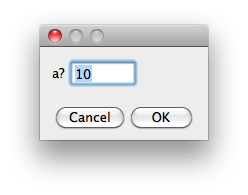
\includegraphics[scale=0.6]{fig/getNumberDialog.png}
\caption{getNumber Dialog} \label{fig_getNUmber}
\end{center}
\end{figure}

The function \textit{getNumber} consists of two parameters (programmers call such parameters "arguments" so we use this word in the reminder of this textbook).
\begin{indentCom}
\textbf{getNumber}(message string, default number)
\end{indentCom}
The first argument is a string wrapped by double quotes (see code 5, line 3
and 4). This string will appear in the dialog window such as shown above. 
Default number will appear in the input field in the dialog window, 
and the user is expected to modifies this default number. 
When OK button is clicked, the number given by the user will be returned to
the macro and then substituted to a variable. In the above case, this could be
either \textit{a} or \textit{b}.
 
To ask a user for providing a string in dialog, following is an example. 
\lstinputlisting[morekeywords={*, getString}]{code/code06.ijm}

The function \textbf{getString} also has two arguments, 
and only the difference is that the user input will be treated as a string. \\

\begin{indentexercise}{1}
Run the code 6 and input 1 for a and 2 for b. What happened? Explain the reason. 
\end{indentexercise}

